%%%%%%%%%%%%%%%%%%%%%%%%%%%%%%%%%%%%%%%%%%%%%%%%%%%%%%%%%%%%%%%%
%%%%%%%%%%%%%%%%%%%%%%%%%%%%%%%%%%%%%%%%%%%%%%%%%%%%%%%%%%%%%%%%
%%%%
%%%% This text file is part of the source of slides for
%%%% `Introduction to High-Performance Scientific Computing'
%%%% by Victor Eijkhout, copyright 2012-2022
%%%%
%%%%%%%%%%%%%%%%%%%%%%%%%%%%%%%%%%%%%%%%%%%%%%%%%%%%%%%%%%%%%%%%
%%%%%%%%%%%%%%%%%%%%%%%%%%%%%%%%%%%%%%%%%%%%%%%%%%%%%%%%%%%%%%%%

\frame{\frametitle{Domain decomposition}
    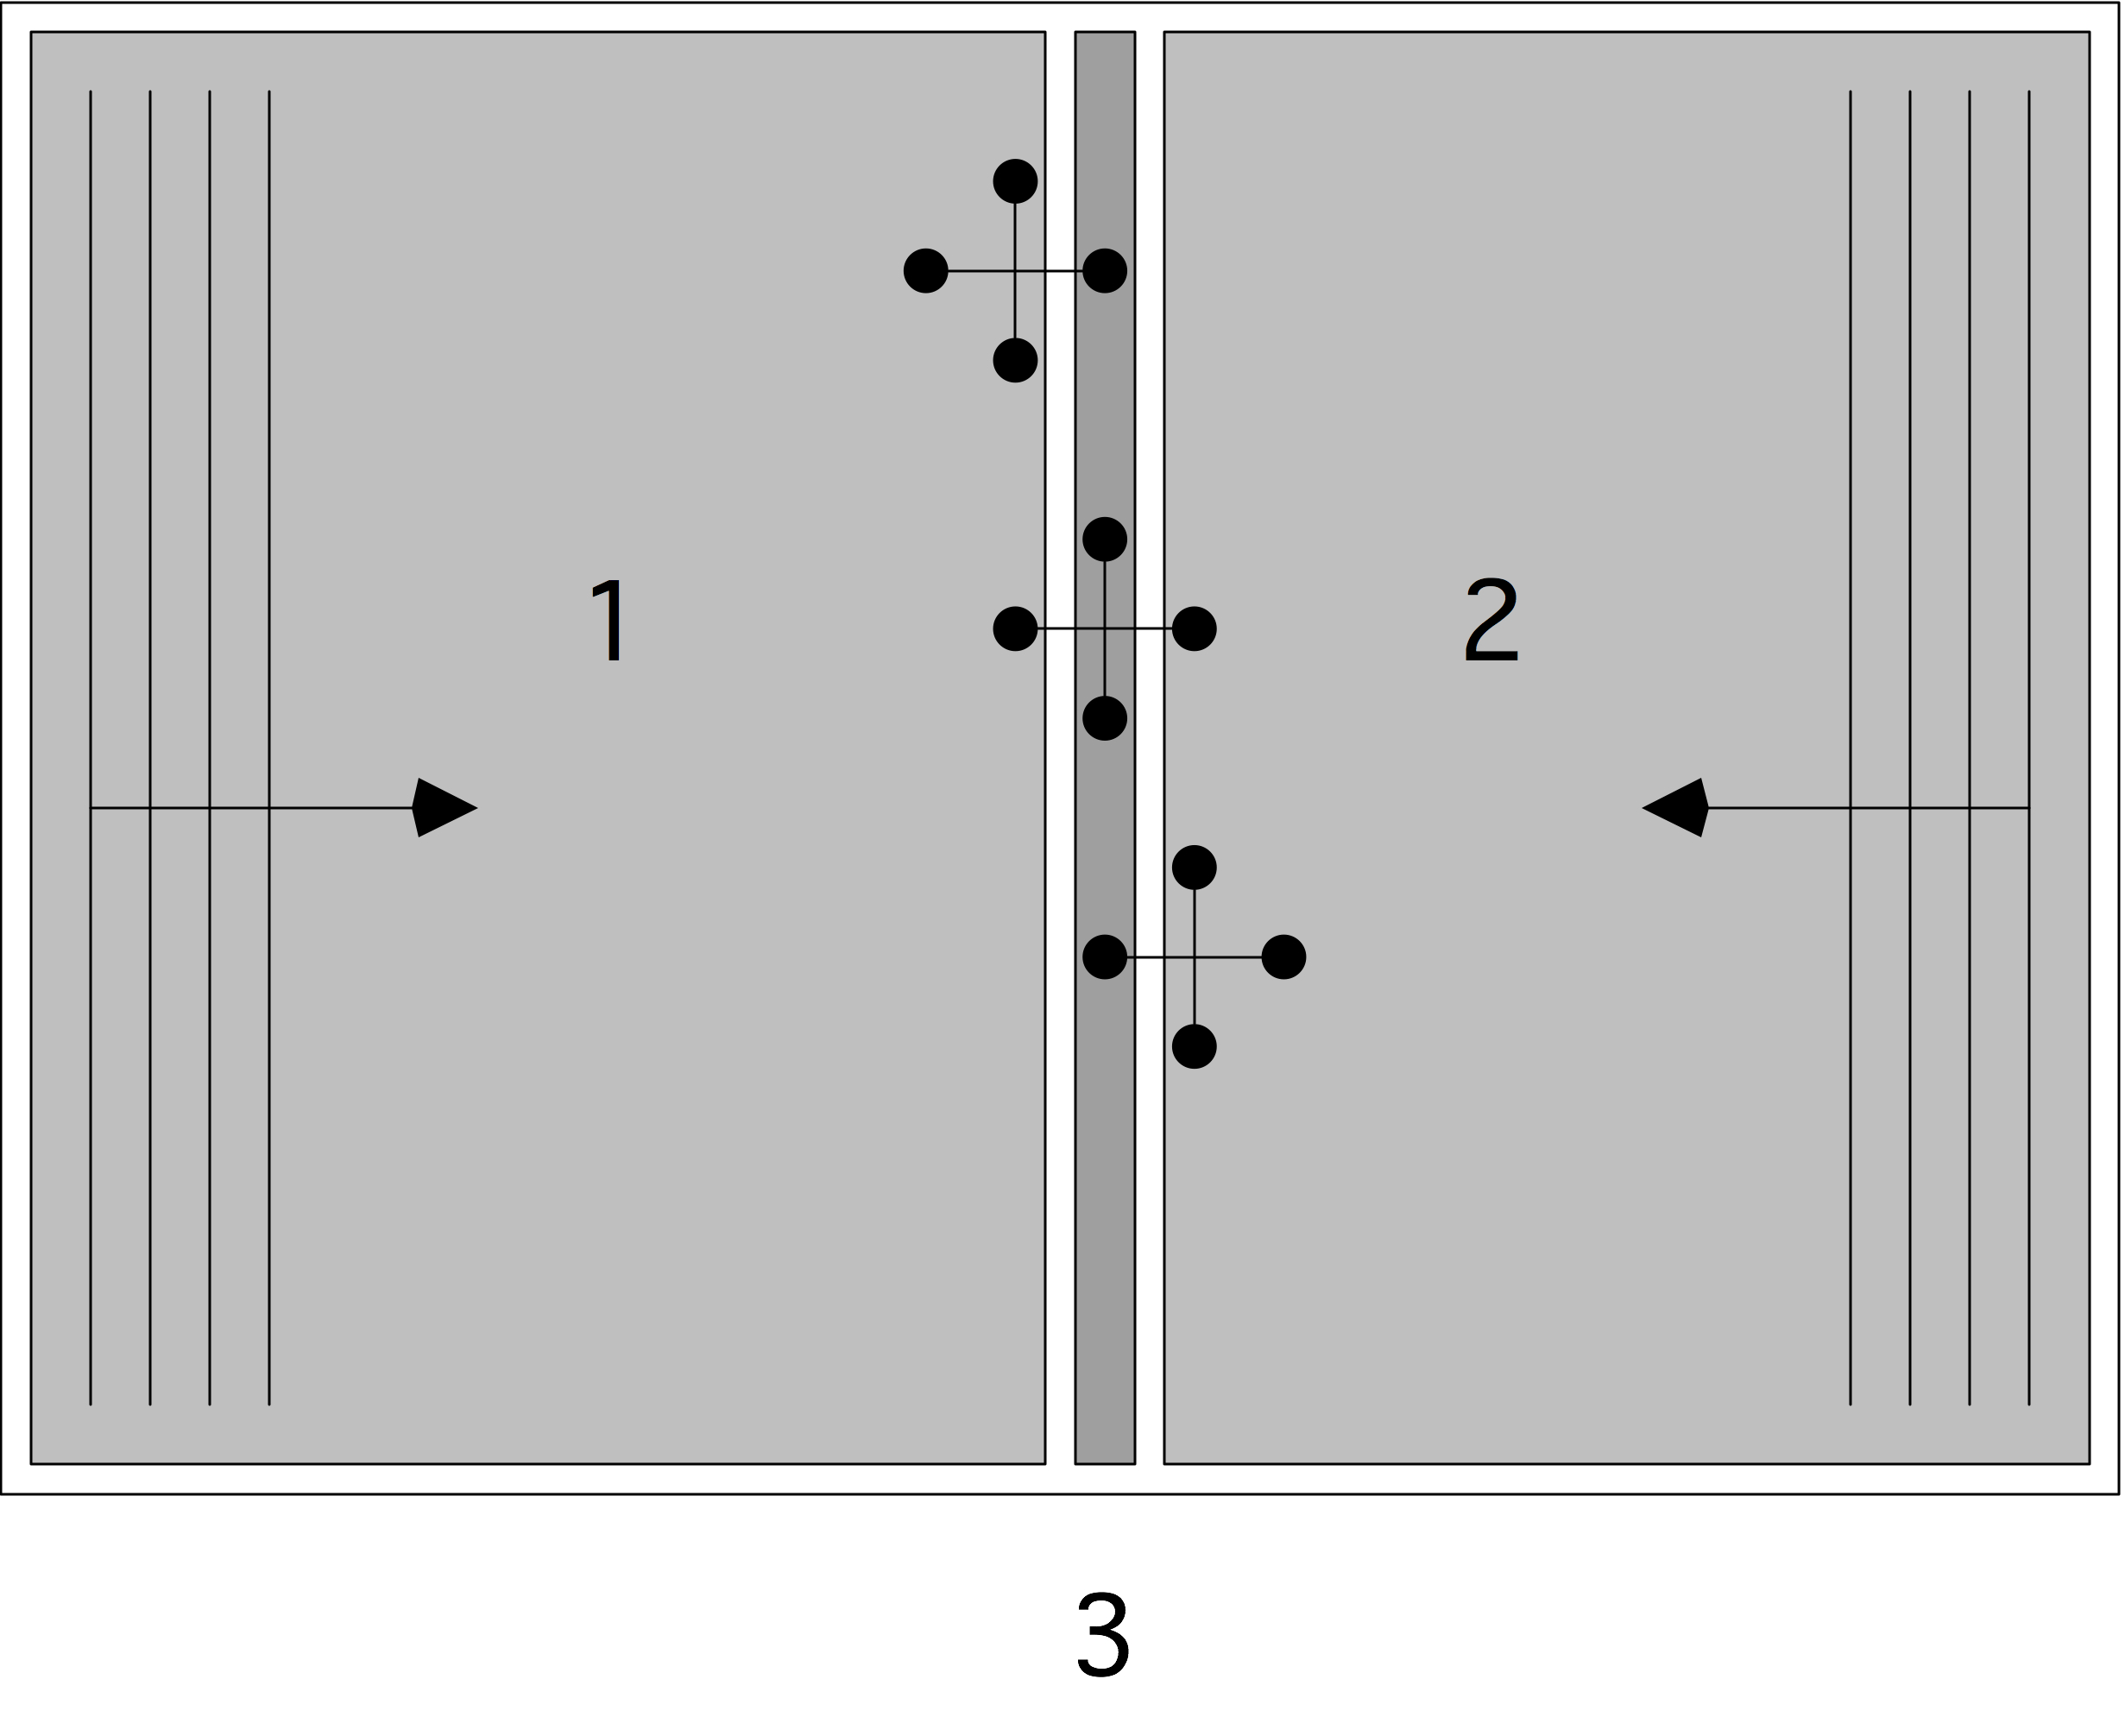
\includegraphics[scale=.1]{domdecomp}
}

\newcommand\Add{A^{\mathrm{DD}}}

\frame{\small
\[
\left(\begin{array}{ccccc|ccccc|c}
  \star&\star &      &      &      &&&&&&0\\
  \star&\star &\star &      &      &&&&&&\vdots\\
       &\ddots&\ddots&\ddots&      &&&\emptyset&&&\vdots\\
       &      &\star &\star &\star &&&&&&0\\
       &      &      &\star &\star &&&&&&\star\\ \hline
  &&&&&\star&\star &      &      &      &0\\
  &&&&&\star&\star &\star &      &      &\vdots\\
  &&\emptyset&&&     &\ddots&\ddots&\ddots&      &\vdots\\
  &&&&&     &      &\star &\star &\star &0\\
  &&&&&     &      &      &\star &\star &\star\\ \hline
  0&\cdots&\cdots&0&\star&0&\cdots&\cdots&0&\star&\star
\end{array}\right)
\begin{array}{c}
  \left.\begin{array}{c}
    \phantom{x}\\ \phantom{x}\\ \phantom{x}\\ \phantom{x}\\ \phantom{x}\\
  \end{array}\right\} \\
  \left.\begin{array}{c}
    \phantom{x}\\ \phantom{x}\\ \phantom{x}\\ \phantom{x}\\ \phantom{x}\\
  \end{array}\right\} \\
  \left.\begin{array}{c}
    \phantom{x}\\ 
  \end{array}\right\}
\end{array}
\begin{array}{c}
  \phantom{x}\\ \phantom{x}\\ (n^2-n)/2\\ \phantom{x}\\ \phantom{x}\\
  \phantom{x}\\ \phantom{x}\\ (n^2-n)/2\\ \phantom{x}\\ \phantom{x}\\
  n
\end{array}
\]
}

\frame{\frametitle{DD factorization}

\[
\begin{array}{l}
\Add=
  \begin{pmatrix}
    A_{11}&\emptyset&A_{13}\\
    \emptyset&A_{22}&A_{23}\\
    A_{31}&A_{32}&A_{33}
  \end{pmatrix}=\\[10pt]
  \begin{pmatrix}
    I\\
    \emptyset&I\\
    A_{31}A_{11}\inv&A_{32}A_{22}\inv&I
  \end{pmatrix}
  \begin{pmatrix}
    A_{11}&\emptyset&A_{13}\\
         &A_{22}&A_{23}\\
    &&S
  \end{pmatrix}
\end{array}
\]
\[ S = A_{33}-A_{31}A_{11}\inv A_{13}-A_{32}A_{22}\inv A_{23} \]
Parallelism\ldots
}

\frame{\frametitle{Graph theory of sparse elimination}

\[ a_{ij} \leftarrow a_{ij}- a_{ik}a_{kk}\inv a_{kj} \]
  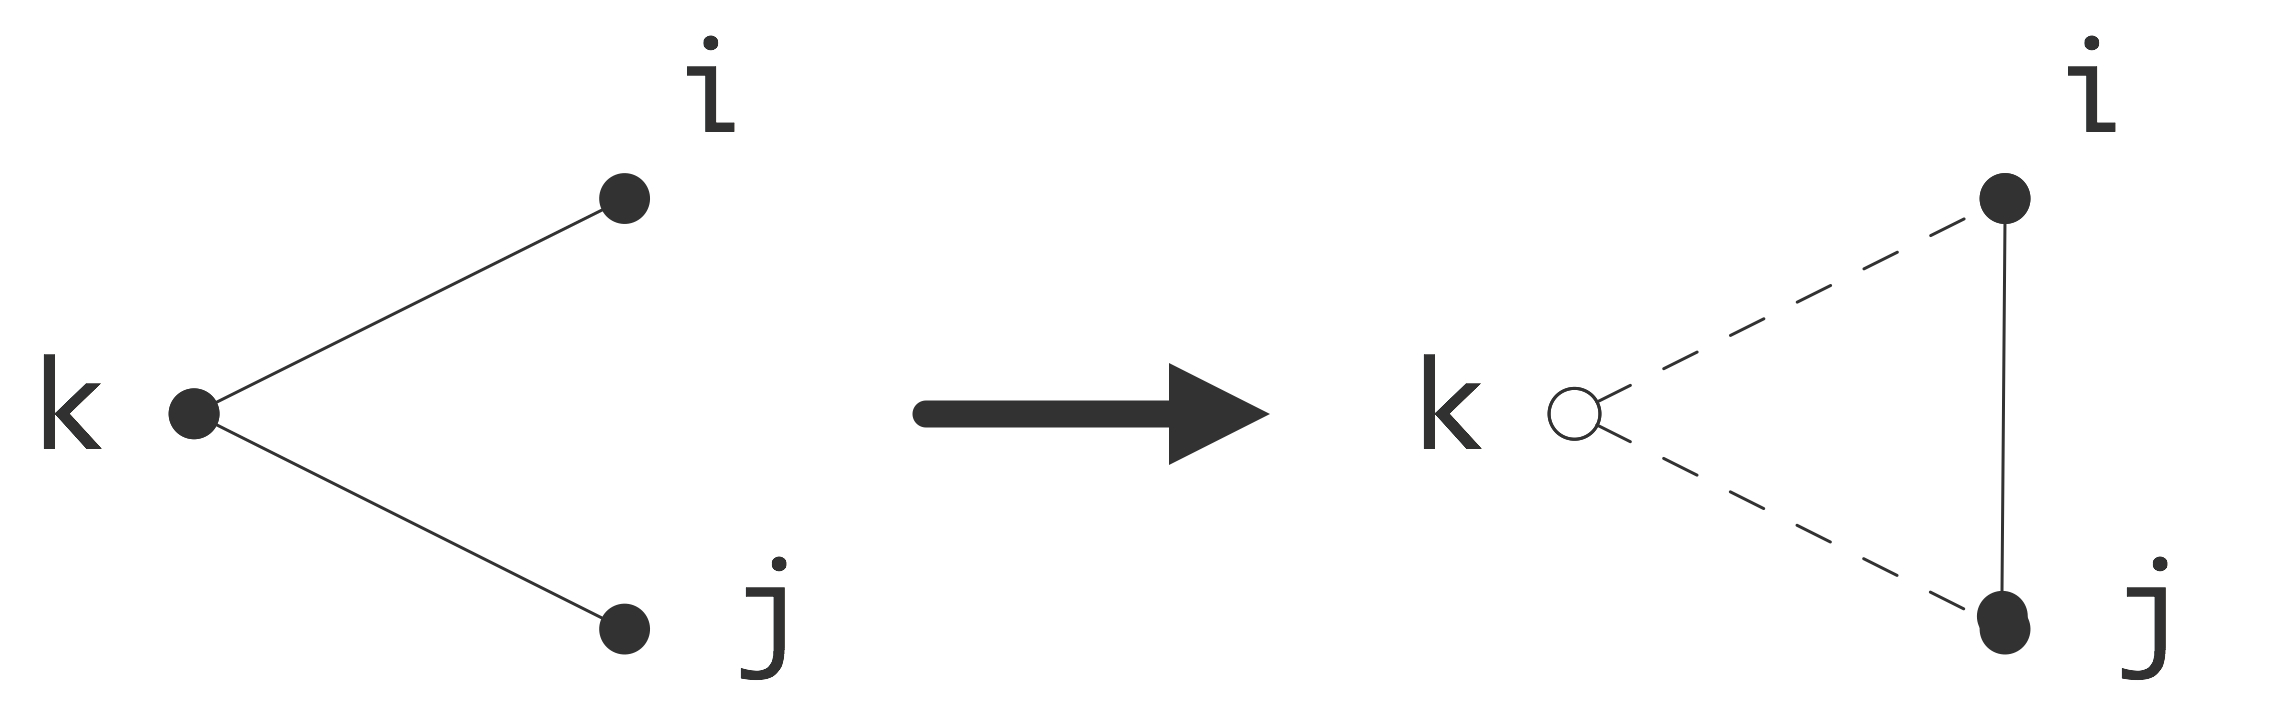
\includegraphics[scale=.12]{ijk-eliminate}
}
\frame{
Apply to
\[ S = A_{33}-A_{31}A_{11}\inv A_{13}-A_{32}A_{22}\inv A_{23} \]

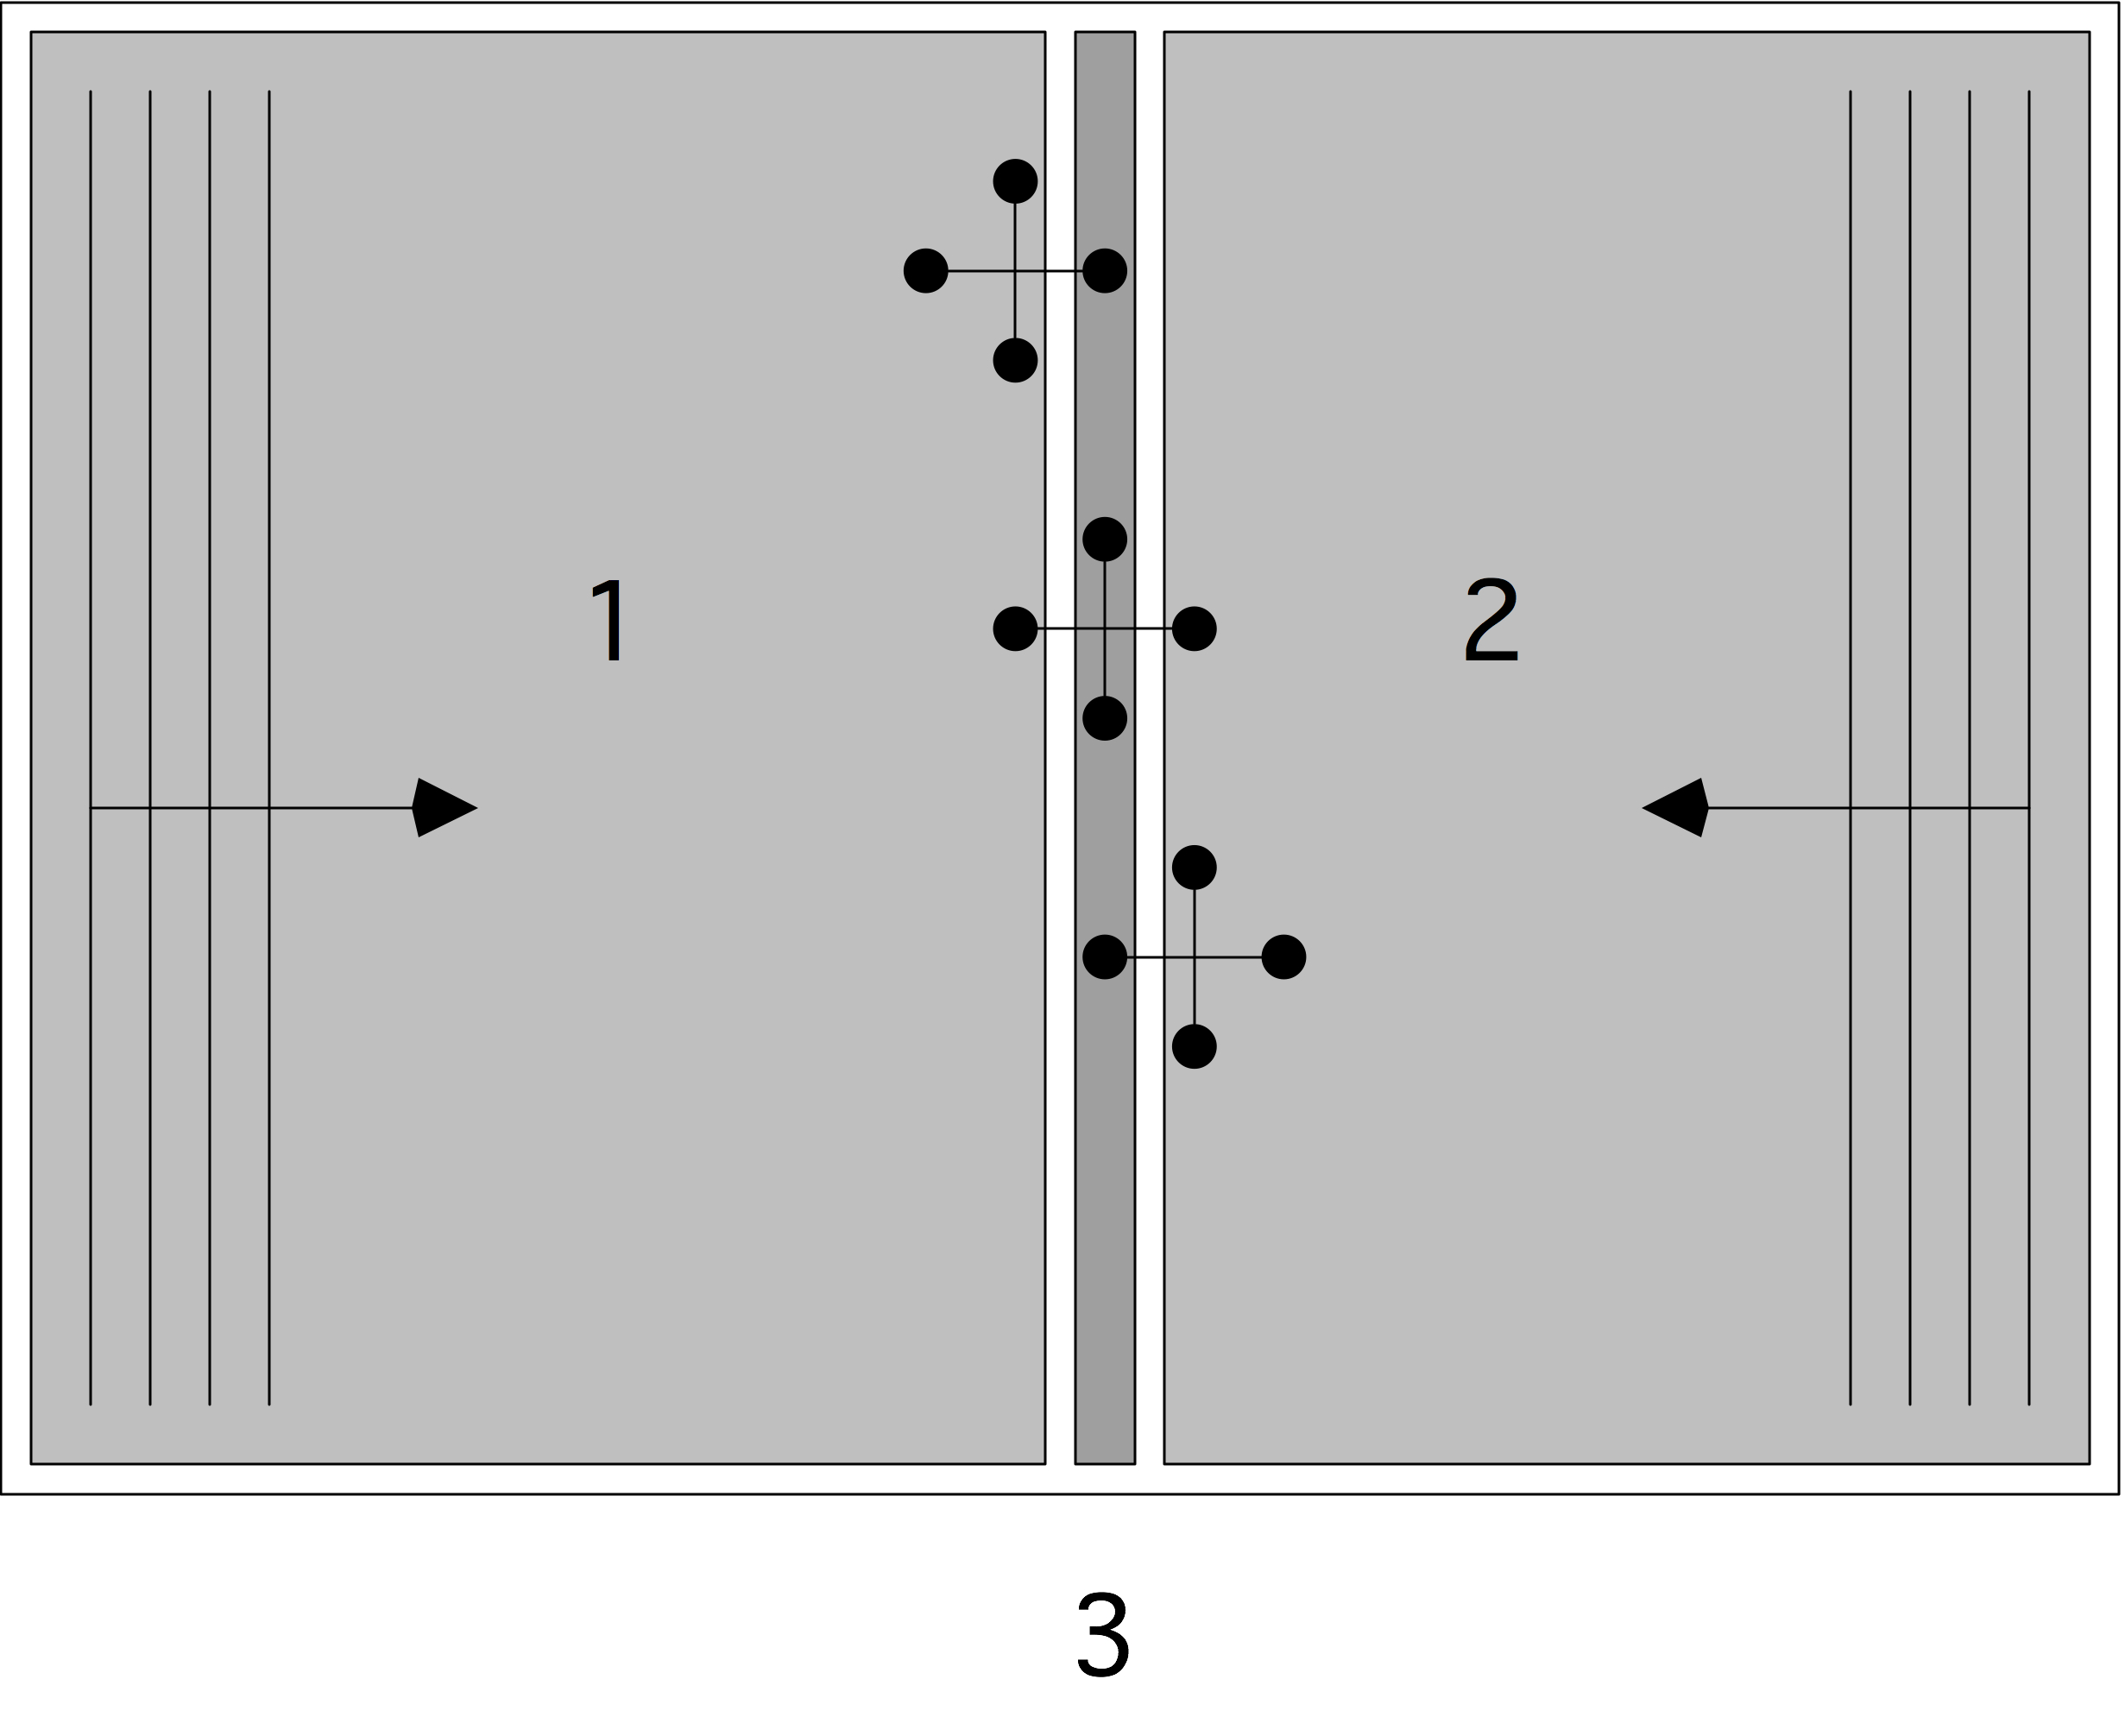
\includegraphics[scale=.08]{domdecomp}

So inductively $S$ is dense
}

\frame{\frametitle{Recursive bisection}
\begin{figure}
  \begin{quote}
    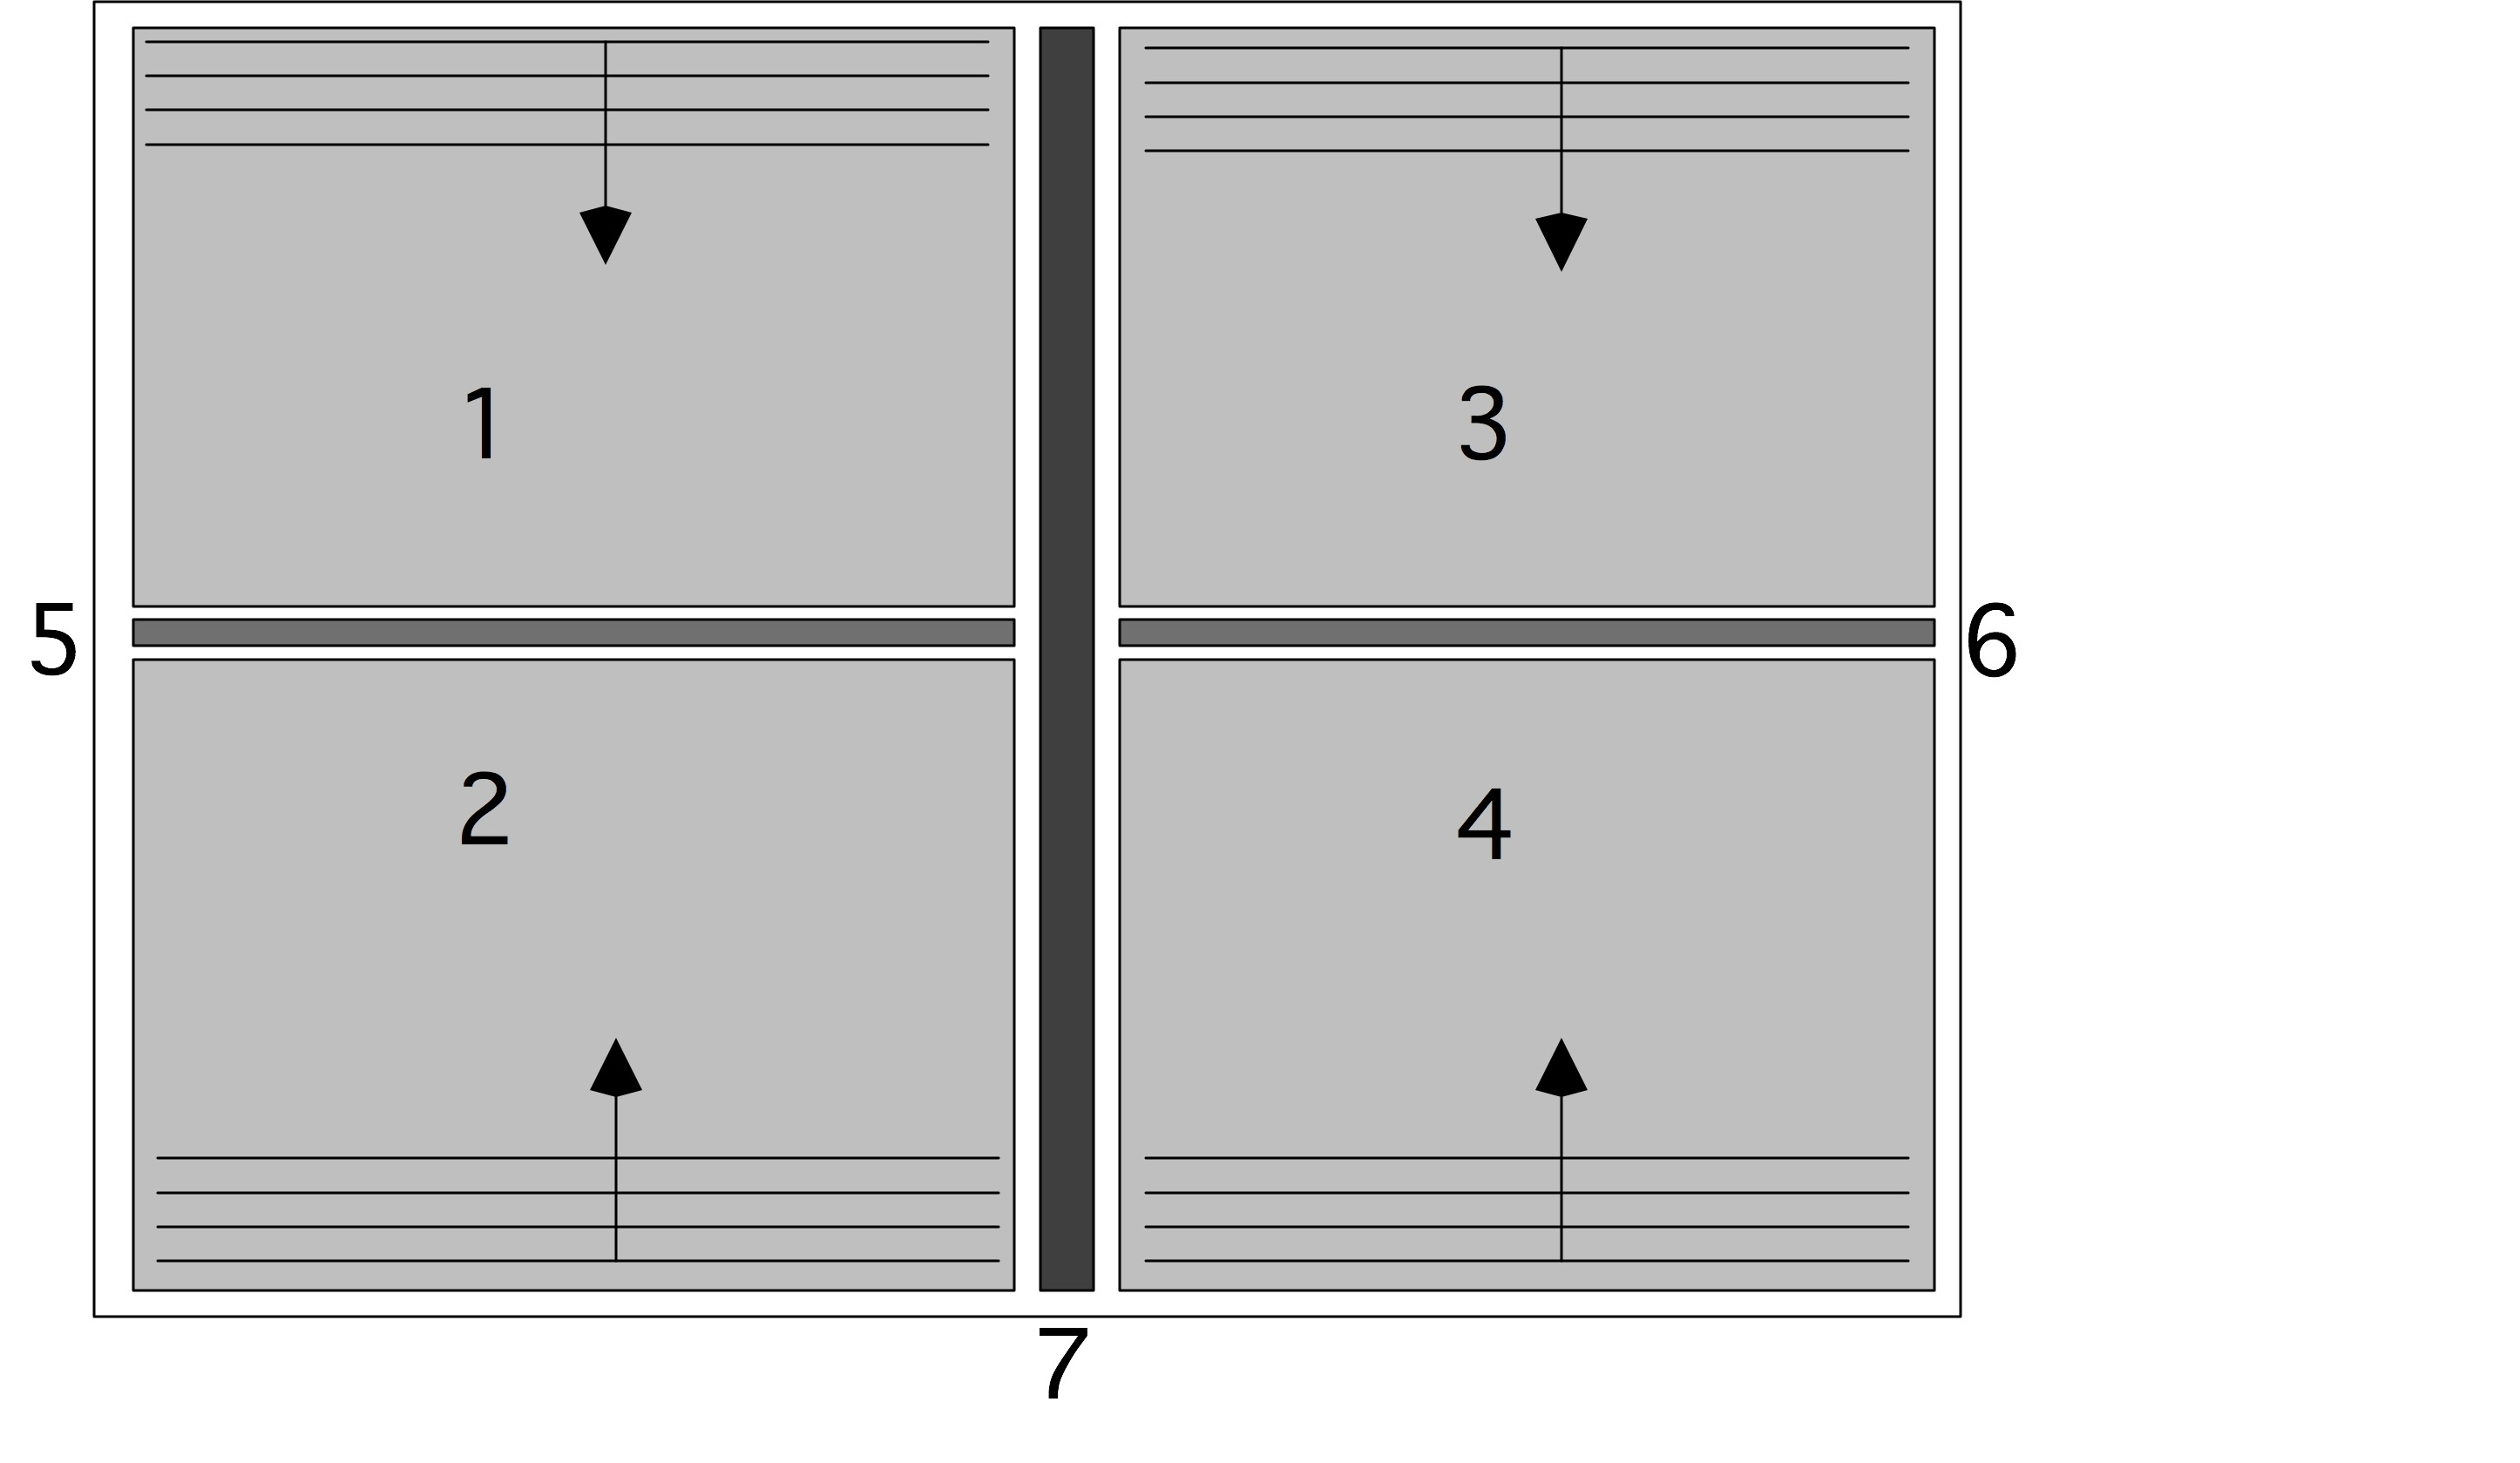
\includegraphics[scale=.11]{domdecomp2}
  \end{quote}
  \caption{A four-way domain decomposition.}
  \label{fig:domdecomp2}
\end{figure}
Parallelism\ldots
}
\frame{
\[
  \Add=
  \left(\begin{array}{ccccccc}
    A_{11}&     &     &     &A_{15}&     &A_{17}\\
         &A_{22}&     &     &A_{25}&     &A_{27}\\
         &     &A_{33}&     &     &A_{36}&A_{37}\\
         &     &     &A_{44}&     &A_{46}&A_{47}\\ 
    A_{51}&A_{52}&    &     &A_{55}&      &A_{57}\\
         &      &A_{63}&A_{64}&    &A_{66}&A_{67}\\
    A_{71}&A_{72}&A_{73}&A_{74}&A_{75}&A_{76}&A_{77}
  \end{array}\right)
\]
The domain/operator/graph view is more insightful, don't you think?
}

\frame{\frametitle{How does this look in reality?}
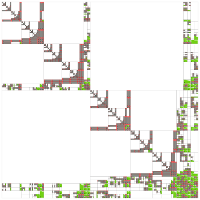
\includegraphics[scale=2.5]{nesteddis}
}

\frame{\frametitle{Complexity}
With $n=\sqrt N$:
\begin{itemize}
\item one dense matrix on a separator of size~$n$, plus
\item two dense matrices on separators of size~$n/2$
\item $\rightarrow 3/2\,n^2$ space and $5/12\,n^3$ time
\item and then four times the above with $n\rightarrow n/2$
\end{itemize}
\[ 
\begin{array}{r@{{}={}}l}
\mathrm{space}&3/2n^2+4\cdot 3/2(n/2)^2+\cdots\\
   & N(3/2+3/2+\cdots)\quad\hbox{$\log n$ terms}\\
   & O(N\log N)
\end{array}
\]
\[ 
\begin{array}{r@{{}={}}l}
\mathrm{time}&5/12n^3/3+4\cdot 5/12(n/2)^3/3+\cdots\\
   & 5/12 N^{3/2}(1+1/4+1/16+\cdots)\\
   & O(N^{3/2})
\end{array}
\]
}

\frame{\frametitle{More direct factorizations}

Minimum degree, multifrontal,\ldots

Finding good separators and domain decompositions is tough in general.
}

%\end{document}
